\section{Magnetoquasistatische Analyse (MQS, Magnetoquasistatic Analysis)}
Die magnetoquasistatische Analyse wird gebraucht um bei Wechselstrom die Ersatzwiderstände eines Gerätes zu berechnen. Weil es sich um langsam ändernde Felder handelt muss der Verschiebungsstrom von Maxwell nicht beachtet werden.  
\subsection{Integralgleichungen}
\begin{tabular}{|p{.30\textwidth} |p{.65\textwidth}|}
	\hline 
	\textbf{Ampèresches Gesetz} \newline
	{\centering\tabbild[width=4cm]{images/ampgesetz.png}\par} & Das Ampèresche Gesetz definiert die Verteilung des magnetischen Feldes durch eine geschlossene Kurve ist der gesamte Strom durch die entsprechende Fläche
	\[ \oint\limits_{(C)}\vec{H}\cdot\vec{dl} = \iint\limits_{(A)}\vec{J}\cdot\vec{dA}\] \newline
	\[ \oint\limits_{(C)}\vec{B}\cdot\vec{dl} = \mu_{0}\iint\limits_{(A)}\vec{J}\cdot\vec{dA} \quad \quad\vec{B}=\mu_{0}\mu_{r}\cdot \vec{H}\]\\
	\hline
	\textbf{Coulombsches Gesetz} \newline
	{\centering\tabbild[width=4cm]{images/quellenfreiheit.png}\par} & Der magnetische Fluss durch eine geschlossene Fläche ist immer Null. Somit sind die magnetische Feldlinien immer geschlossen. Es gibt keine magnetische Monopole. Das magnetische Feld ist Quellenfrei \newline
	\[ \oiint\limits_{(A)}\vec{B}\cdot\vec{dA} = 0\]\\
	\hline
	\textbf{Faradaysches Induktionsgesetz}
	{\centering\tabbild[width=4cm]{images/faradaygesetz.png}\par} & Der zeitabhängige magnetische Fluss induziert elektrische Spannung in der vom Fluss durchflossenen Spule.\newline
	\[u_{i}=-\frac{\partial \Phi_{m}}{\partial t}\] \newline
	\[\Phi_{m}=\oiint\limits_{(S)} \vec{B}\cdot \vec{dS}\quad und \quad u_{i}=\oint \limits_{(C)}\vec{E}\cdot \vec{dl}\]\newline
	\[\oint \limits_{(C)}\vec{E}\cdot \vec{dl}= - \frac{\partial}{\partial t} \oiint\limits_{(S)} \vec{B}\cdot \vec{dS}\]\\
	\hline
\end{tabular}
\clearpage
\pagebreak
\subsection{Differenzialgleichungen der magnetoquasostatischen Analyse}
\begin{tabular}{|p{.45\textwidth} |p{.45\textwidth}|}
	\hline
	\textbf{Differenzialgleichung der Durchflutung}\newline
	\[\rotation \vec{H}=\nabla \times \vec{H}=\vec{J}\]&
	\textbf{Poissongleichung}\newline
	Die obige Gleichung wird mit Umweg über das Vektorpotential A des Magnetfeldes gelöst
	\[\vec{E}=-\dfrac{\partial \vec{A}}{\partial t}\]
	\[\Delta\vec{A}-\mu_{0}\sigma \dfrac{\partial \vec{A}}{\partial t}=-\mu_{0}\vec{J}\]\\
	\hline
\end{tabular}
\subsection{Randbedingungen}
\begin{itemize}
	\item Magnetische Isolierung $\vec{n} \times \vec{A} =0$
	\item Der Rand zwischen zwei Materialien $\vec{n} \times \vec{A_{1}}=\vec{n} \times \vec{A_{2}}$
\end{itemize}
\subsection{Randwertproblem}
\begin{minipage}{9cm}
	\begin{itemize}
		\item Zeitbereich: $\Delta\vec{A}-\mu_{0}\sigma \dfrac{\partial \vec{A}}{\partial
		 t}=-\mu_{0}\vec{J}$
		\item Frequenzbereich: $\Delta\vec{A}-j\omega\mu_{0}\sigma\vec{A}=-\mu_{0}\vec{J}$
		\item $\vec{n} \times \vec{A} =0$
	\end{itemize}	
\end{minipage}
\begin{minipage}{8cm}
	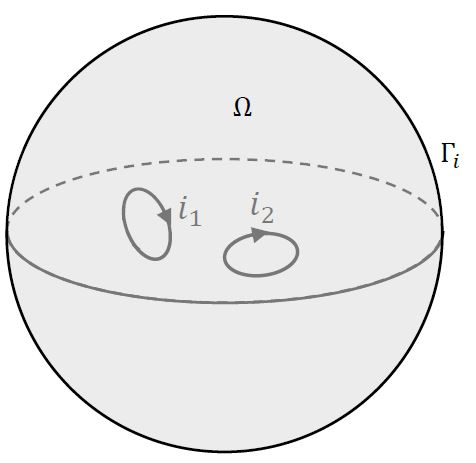
\includegraphics[width=4cm]{images/Randwertproblem.jpg}
\end{minipage}
\clearpage
\pagebreak
